\chapter{Procesy zachodzące w systemie}
\section{Rejestracja}
Rejestraccja użytkownika w systemie realizowana jest za pomocą zewnętrznego serwisu \textit{Auth0}. 

\begin{figure}[h]
	\centering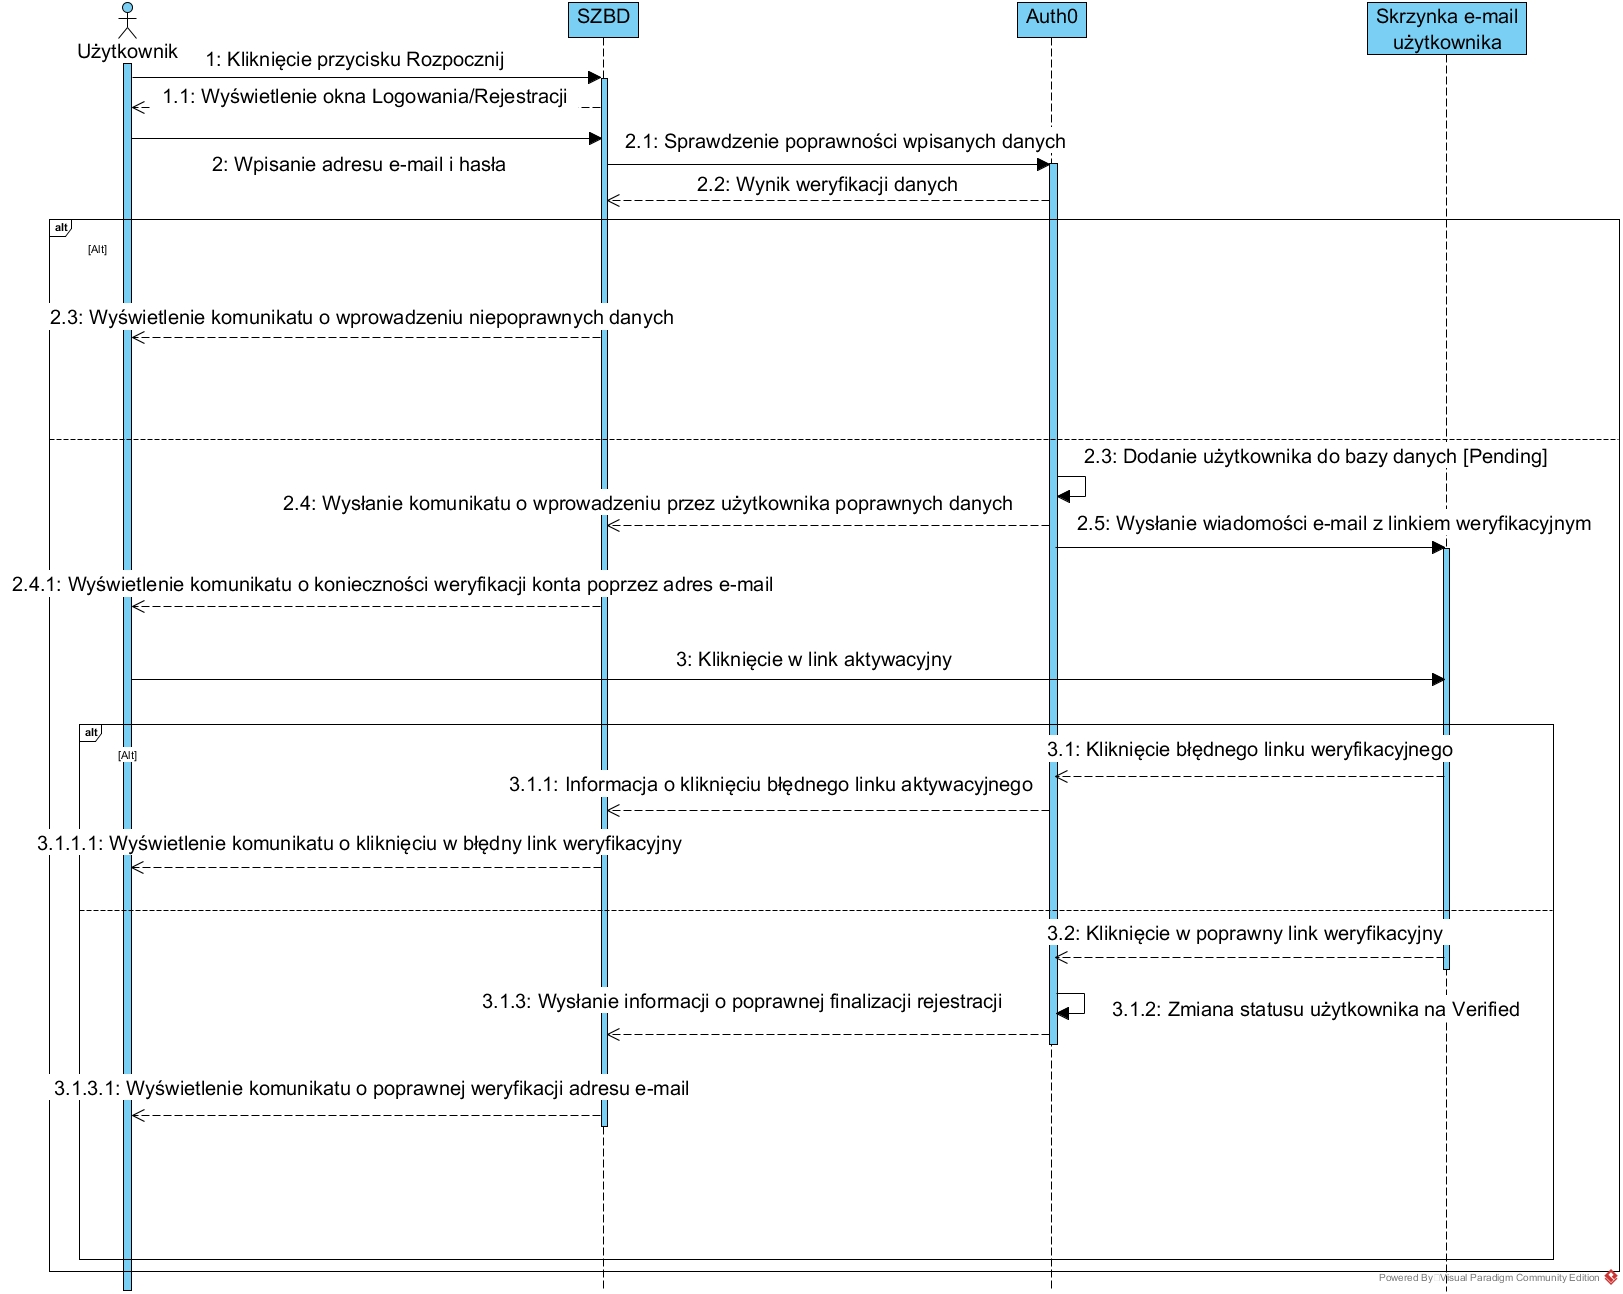
\includegraphics[scale=0.25]{images/sequence_diagram3.jpg}
	\caption{Diagram sekwencji przedstawiający proces rejestracji nowego użytkownika}
	\label{Rys:registration}
\end{figure}

\newpage

\section{Logowanie}
Logowanie użytkownika w systemie realizowane jest za pomocą zewnętrznego serwisu \textit{Auth0}.

\begin{figure}[h]
	\centering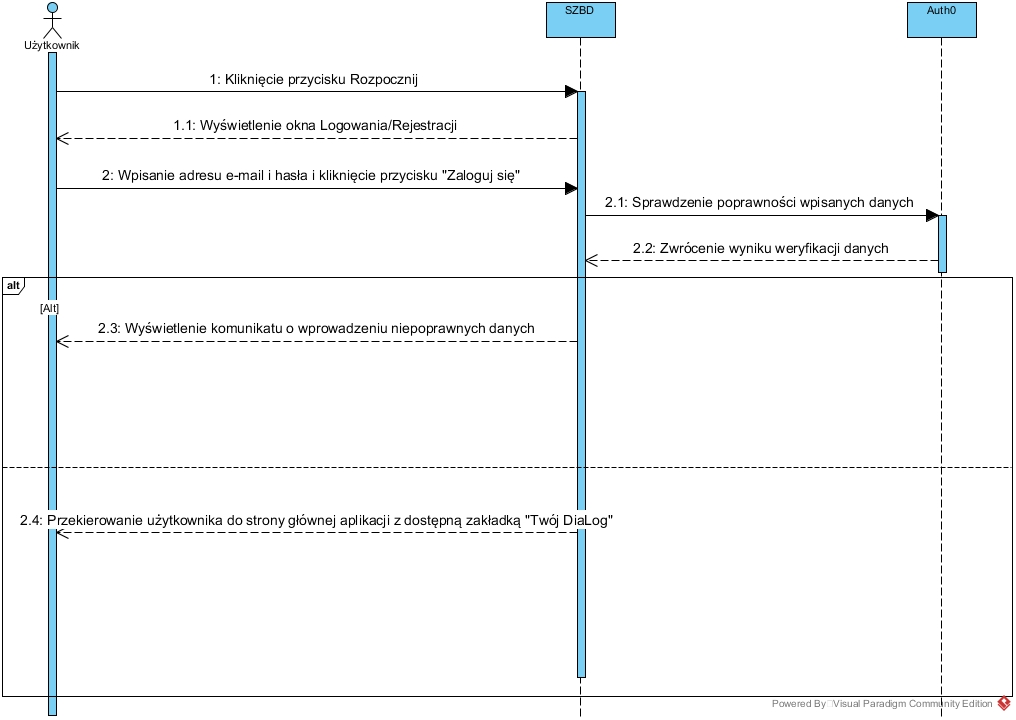
\includegraphics[scale=0.4]{images/sequence_login.jpg}
	\caption{Diagram sekwencji przedstawiający proces logowania użytkownika}
	\label{Rys:login}
\end{figure}

\section{Wprowadzanie i edycja informacji o profilu}
Użytkownik ma możliwość wprowadzania i późniejszej edycji danych dotyczących informacji o~ profilu. Odbywa się to poprzez wypełnienie formularza. Użytkownik (poprzez odpowiednie wypełnienie pól formularza) określa: 
\begin{itemize}
	\item imię,
	\item nazwisko,
	\item PESEL,
	\item posiadanie opiekuna,
	\item adres zamieszkania (ulica, numer domu, miasto, kod pocztowy),
	\item numer telefonu,
	\item aktualny model glukometru,
	\item poprzedni modelu glukometru,
	\item numer seryjny glukometru.
\end{itemize}
W przypadku chęci edycji tych danych wystarczy zastąpić je w odpowiednim polu i kliknąć przycisk \textit{Zapisz}.

\section{Wprowadzanie i edycja danych medycznych}
Użytkownik ma możliwość wprowadzania i późniejszej edycji danych medycznych. Odbywa się to poprzez wypełnienie formularza. Użytkownik (poprzez odpowiednie wypełnienie pól formularza) określa: 
\begin{itemize}
	\item typ cukrzycy,
	\item rok zachorowania,
	\item rodzaj insuliny,
	\item przyjmowane leki,
	\item inne leki i insuliny,
	\item wzrost,
	\item wagę,
	\item poziom współczynnika HbA1c.
\end{itemize}
W przypadku chęci edycji tych danych, podobnie jak w poprzednim przypadku należy zastąpić je odpowiednimi informacjami i wybrać przycisk \textit{Zapisz}.

\section{Dodawanie nowego pomiaru}
Użytkownik ma możliwość dodania nowego pomiaru. Czynność ta odbywa się poprzez kliknięcie przycisku \textit{Nowy pomiar}. Po wykonaniu tej czynności ukazuje się okno modalne z odpowiednimi polami do wypełnienia:
\begin{itemize}
	\item data i godzina pomiaru,
	\item glikemia,
	\item moment pomiaru,
	\item krótka notatka.
\end{itemize}
Po wypełnieniu wszystkich pól formularza należy kliknąć przycisk \textit{Dodaj}. Okno modalne zostaje wówczas automatycznie zamknięte, a nowo prowadzone dane zostają dodane do sekcji wykresów i~ tabeli podsumowań. 

\section{Dostęp do wykresów i tabeli zestawień}
Użytkownik w każdym momencie może uzyskać dostęp do wykresów i tabeli zestawień poprzez wybranie pozycji menu \textit{Twoja glikemia}. Wykresy oraz dane zawarte w tabeli generowane są w~ sposób automatyczny po dodaniu nowej wartości pomiaru. 

\section{Obliczanie wartości BMI}
Użytkownik w dowolnym momencie może sprawdzić swoją wartość współczynnika BMI (\textit{Body Mass Index}) poprzez wybranie z menu bocznego pozycji \textit{Kalkulatory}, a następnie wprowadzenie swojej wagi oraz swojego wzrostu i kliknięcie przycisku \textit{Oblicz}. W momencie wyświetlenia wyniku program podpowiada użytkownikowi jak współczynnik BMI odwzorowuje się na jego aktualnej sylwetce i kondycji zdrowotnej:
\begin{itemize}
	\item niedowaga,
	\item waga prawidłowa,
	\item nadwaga,
	\item otyłość I stopnia,
	\item otyłość II stopnia,
	\item otyłość III stopnia.
\end{itemize}

\section{Obliczanie wartości wymienników węglowodanowych i~ białkowo-tłuszczowych na podstawie dostępnej bazy produktów}
Użytkownik ma możliwość obliczenia współczynnika wymienników węglowodanowych oraz wymienników białkowo-tłuszczowych na podstawie dostępnej bazy produktów, która może być rozwijana przez użytkowników. W pierwszej kolejności użytkownik wybiera produkt z pola formularza z~ wbudowanym inteligentym modułem wyszukiwania produktów. W następnej kolejności użytkownik wybiera wagę produktu (domyślna wartość to 100 gram). W tabeli zawartej poniżej formularza użytkownik ma dostęp do tabeli makroskładników danego produktu:
\begin{itemize}
	\item kilokalorie produktu [kcal],
	\item ilość białka [g],
	\item ilość tłuszczu [g],
	\item ilość węglowodanów [g],
	\item ilość błonnika [g],
	\item wielkość porcji [g],
	\item wartość współczynnika wymienników węglowodanowych,
	\item wartość współczynnika wymienników białkowo-tłuszczowych.
\end{itemize}
Wartości zawarte w tabeli są dynamicznie zmieniane w zależności od wprowadzonej gramatury produktu.

\section{Dodawanie produktów do bazy danych produktów}
Użytkownik ma możliwość dodania produktu do bazy danych produktów. Odbywa się to za pomocą wypełnienia odpowiednich pól formularza:
\begin{itemize}
	\item nazwa produktu,
	\item kalorie [kcal],
	\item białko [g],
	\item tłuszcz [g],
	\item węglowodany [g],
	\item błonnik [g],
	\item porcja [g].
\end{itemize}
Aby zatwierdzić zmiany należy kliknąć przycisk \textit{Zapisz}. Produkt automatycznie zostanie dodany do bazy danych i w sposób dynamiczny będzie dostępny w wyszukiwarce produktów. 

\section{Wysłanie wiadomości e-mail z zapytaniem dotyczącym serwisu przy użyciu modułu do wysyłania poczty elektronicznej}
Użytkownik ma możliwość wysłania wiadomości e-mail do administracji strony poprzez wypełnienie odpowiednich pól formularza dostępnych na stronie startowej:
\begin{itemize}
	\item imię,
	\item e-mail,
	\item temat,
	\item treść wiadomości.
\end{itemize}
W celu zatwierdzenia wiadomości e-mail należy kliknąć przycisk Wyślij. 

\section{Diagram przypadków użycia}
W poniższej sekcji, na rysunku \ref{Rys:useCaseDiagram} zaprezentowany został diagram przypadków użycia dla każdego z aktorów.

\begin{figure}[h]
	\centering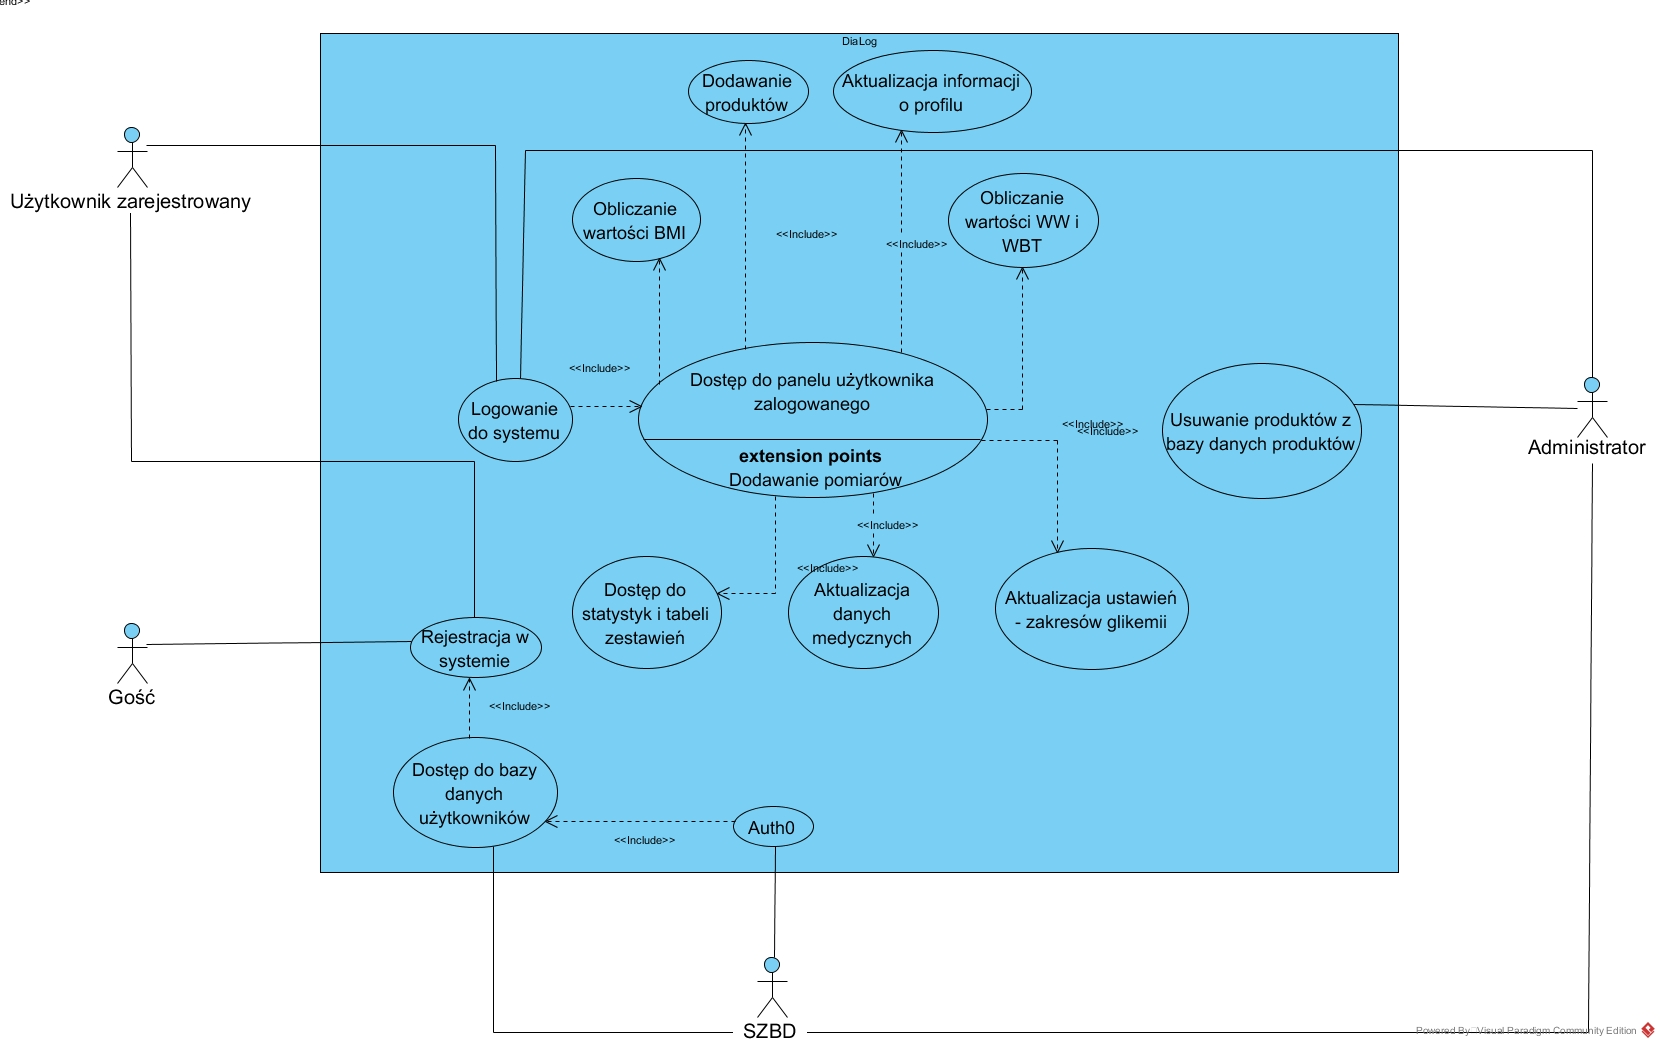
\includegraphics[angle=90, scale=0.4]{images/use_case_diagram.jpg}
	\caption{Diagram przypadków użycia dla aktorów aplikacji}
	\label{Rys:useCaseDiagram}
\end{figure}
